\section{Confidence Estimation and Anomaly Rebuttal}
\label{sec:conf_contextualization}

The use of \ac{DL} models in critical applications - such as autonomous driving, medical diagnosis, and, in the context of this work, large-scale agricultural monitoring - makes the reliability of these models a primary concern. It is not enough to simply search for models with high evaluation metrics; it is essential that such models be capable of assessing the reliability of their own predictions and identifying when a prediction is subject to significant uncertainty.

Historically, the standard approach to estimating the confidence of a classification model has been to use Maximum Class Probability (MCP), obtained directly from the softmax layer of the network, which is usually the last layer of a classification Deep Neural Network. However, the literature points out that MCP has significant conceptual flaws for confidence prediction. The main problem lies in the fact that modern neural networks are overconfident~\citep{NEURIPS2021_61f3a6db,pmlr-v162-wei22d}, assigning high probabilities even to incorrect predictions. This results in considerable overlap in the confidence distributions between hits and misses, making the raw use of network outputs poor confidence rankings.

\cite{corbiere2019addressing} proposes ConfidNet, an auxiliary neural network that estimates the reliability of a classification model's predictions, proposing the use of True Class Probability (TCP) as a target metric to distinguish failures, since the output of the last layer tends to be overconfident, even in incorrect predictions. In terms of methodology, ConfidNet is trained on the feature extraction layers of an already trained classifier, whose weights are kept frozen during the initial phase. Subsequently, the backbone of the original classifier is copied and its weights are fine-tuned together with the auxiliary confidence prediction network. The network minimizes an MSE calculated between the confidence predicted by ConfidNet and the probability that the original classifier assigned to the ground truth of that specific sample. As for the network architecture itself, it consists of linear layers with ReLU activation, ending with a sigmoid activation to ensure that the output is in the range of 0 and 1. This technique can be applied to any classifier network and will therefore be used as a baseline in this work.

While traditional classification assumes a closed set scenario, where all possible classes are known during training, the \acf{OSR} scenario, i.e., open set, assumes that the model must correctly classify known classes while identifying samples belonging to unknown classes~\citep{10582552}. \ac{OSR} techniques can be adapted to the confidence problem by treating incorrect predictions as anomalies or outliers in the model's embedding space. In this context, \acf{GeMOS}~\citep{vendramini2021opening} proposes a plug-and-play framework that couples a \ac{GMM} per predicted class on the embeddings of the network's intermediate layers extracted by a supervised \ac{CNN} trained on a closed set, with the training of the \ac{GMM}s limited to the training samples for which the network made correct predictions. During inference, the model calculates a likelihood score that indicates how well a sample fits the distribution of the predicted class, where low likelihood values suggest that the sample is an anomaly (or a classification error). Similarly, \cite{10418501} also suggests using \ac{GMM}s to model the distribution of embeddings, but using superpixels for \ac{OSR} in semantic segmentation.

\begin{figure}[ht!]
\centering
\caption{Comparison between closed set and open set classification.}
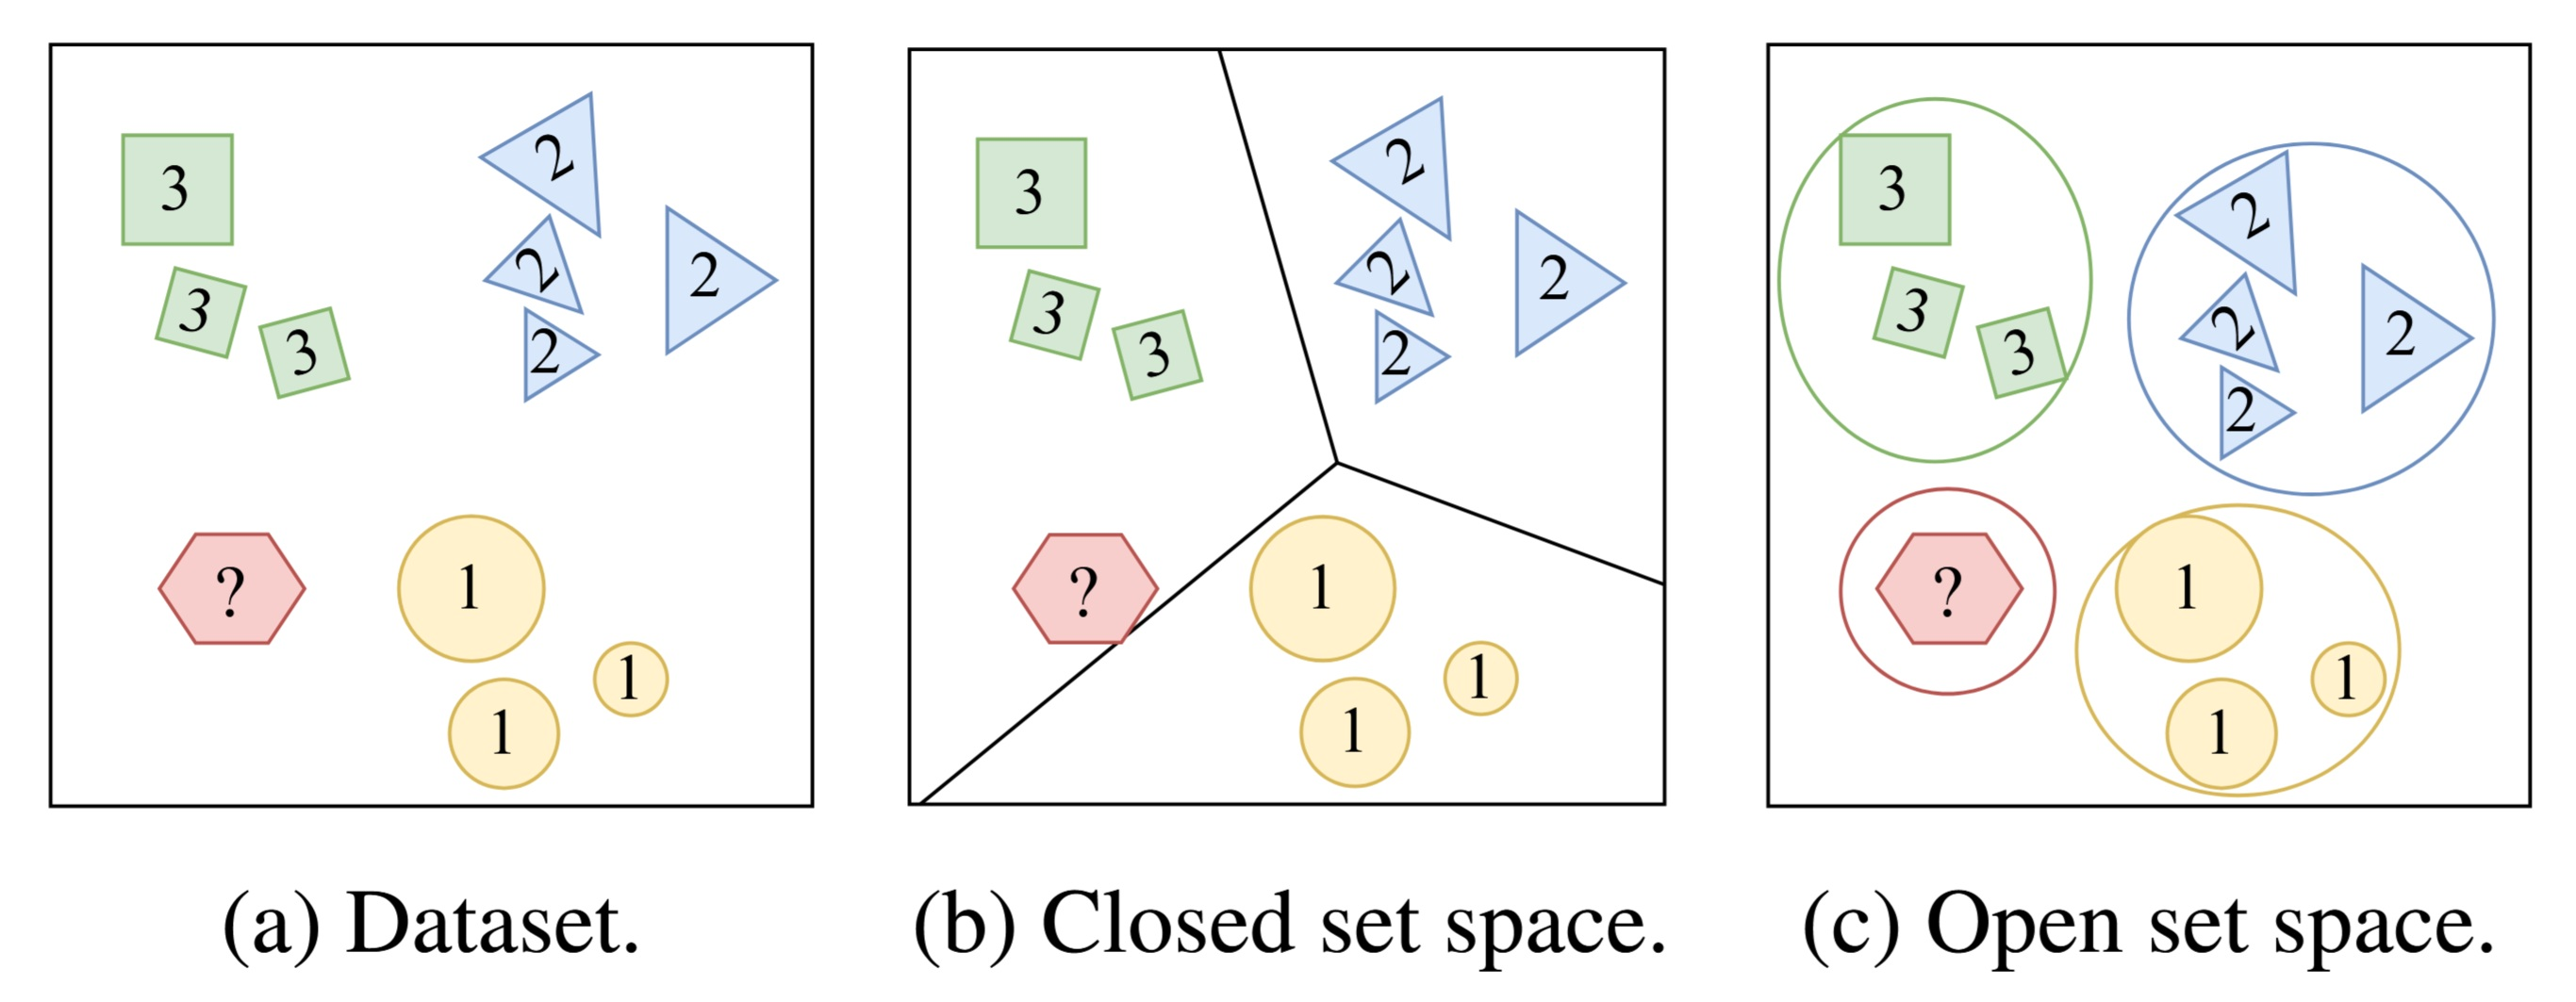
\includegraphics[width=0.95\linewidth]{figures/3_theoretical_background/gemos.jpg}
\fignote{One should notice that, in Closed Set (b) the sample ``?'', from a new class, would be classified erroneously as class 3. In Open set (c), the sample would be classified as an ``unknown'' class - Adapted from \cite{vendramini2021opening}}
\label{fig:osr}
\end{figure}

In addition to generative models on embeddings, other techniques seek semantic consistency by reconstructing the input data. The Conditional Reconstruction for Open-set Semantic Segmentation (CoReSeg) method~\citep{9897407} uses a conditional reconstruction approach, where the network attempts to reconstruct the input image only on known classes, which are those present in the training dataset. The premise is that objects of known classes will be well reconstructed, while unknown objects or classification errors will result in a high reconstruction error.